%loads the class that provides the titlepage and some general packages.
\documentclass{UniVieCS_Thesis} 

%add the additional packages and macros that you want to use
\input{A) Front Matter/packages_macros}
\microtypesetup{expansion=false} % Fix: font expansion only works with scalable fonts

% important update for glossaries, before document 
\loadglsentries{C) Back Matter/acronyms.tex}
\loadglsentries{C) Back Matter/glossary.tex} 
\makeglossaries %https://www.overleaf.com/learn/latex/glossaries

%shows fixme notes
%\fxsetup{status=draft} % comment/delete this line if you want to your final output

\usepackage[ngerman, british]{babel} %if changed to \usepackage[ngerman]{babel} "Table of contents" changes to "Inhaltsverzeichnis", "abstract" becomes "Zusammenfassung" and "references" is translated to "Literatur".


%remove all the things you don't need and add all the things you need. you can also change the order of the elements at your will.
\begin{document}

%Start with front matter

%Choose the titlepage you want to use

%\input{A) Front Matter/titlepage_msc} %Creates the titlepage
\input{A) Front Matter/titlepage_bsc} %Creates the titlepage
%\input{A) Front Matter/titlepage_phd} %Creates the titlepage

\clearpage
\frontmatter{}
%\input{A) Front Matter/acknowledgements} %adds the aknowledgements
%Please consider the following section of the "Formvorschriften für die gedruckte Version"
%Im Anhang ist eine Zusammenfassung (Abstract) mitzubinden.
%Ist die Arbeit in einer Fremdsprache verfasst, ist im Anhang jedenfalls eine deutsche Zusammenfassung mitzubinden.
\chapter{Abstract}
The kinematics of the Taurus molecular cloud complex have so far mainly been studied through the
discrete velocities of its individual members. A full three-dimensional space velocity, however,
requires a radial velocity, which is available for only about one third of the known members, while
proper motions are measured for essentially all of them. This thesis therefore reconstructs a
continuous three-dimensional velocity field of the complex from the full stellar sample, using
information field theory as implemented in \texttt{NIFTy}. Each velocity component is modeled as a
correlated field on a grid of $3~\mathrm{pc}$ cells spanning $126 \times 69 \times 81~\mathrm{pc}$,
with a power spectrum inferred from the data. The stars enter the
likelihood through their observables, so that a star without a radial velocity still constrains the
field within the plane of the sky while its missing component is supplied by the spatial correlation
with its neighbors. The input catalog consists of 557 members identified with \texttt{SigMA} in
Gaia~DR3 astrometry, of which 123 contribute a radial velocity after quality cuts.

The reconstruction reproduces the bulk motion of the complex, resolves velocity differences between
its subgroups and recovers an age--velocity gradient that is already visible in the stellar data.
Both the mean motion and the quantities derived from the field, however, depend strongly on the
individual run of the algorithm: repetitions with a different random seed, with different quality cuts or with a
modified model yield mean motions that scatter by several $\mathrm{km\,s^{-1}}$, while the posterior
uncertainty within a single run stays far below that. A comparison of several such runs is therefore
used to separate features demanded by the data from artifacts of a particular reconstruction. The
residuals between the stars and the field expose the central limitation of the model: the peculiar
motion of a star has nowhere to go but into the field itself. Granting the stars a common intrinsic
velocity dispersion, inferred alongside the field, brings the weighted residuals of the proper
motions from several standard deviations down to below one, although it does not bring the field
closer to the data.
 % adds the abstract
%\input{A) Front Matter/kurzfassung} %adds the "Kurzfassung"in german.
\pagebreak

\microtypesetup{protrusion=false}
\tableofcontents{}
% Use an optional list of tables / figures / algorithms / listings(code).
%\listoftables
%\listoffigures
\cleardoublepage{}
%\listofalgorithms
\addcontentsline{toc}{chapter}{List of Algorithms}
\cleardoublepage{}
%\lstlistoflistings
\cleardoublepage{}
\microtypesetup{protrusion=true}

\pagebreak

%add your chapters here
\mainmatter{}
\chapter{Introduction}
The local neighborhood of our sun is a region containing various interesting subjects worth being studied.
The sun and earth are located approximately in the center of a vast region of relatively empty space containing
high-temperature plasma which is surrounded by a shell of interstellar gas and dust. Most star-forming regions
near the sun are located on the surface of this shell, which is called the Local Bubble. It is thought to
be the result of a burst of supernovae occuring near the center around 14 Myr ago. The likely perpetrators of this
event were around 15 young stellar objects in the Scorpius-Centaurus (Sco-Cen) OB association. Sco-Cen has since moved away
from the center of the Local Bubble, but the resulting expansion of the shell has continued to push the interstellar
medium~(ISM) outwards and has triggered the creation of new star-forming regions on the surface of the bubble.
One of these regions is the Taurus molecular cloud, which is the subject of this thesis \cite{Zucker2022}.
\chapter{Taurus Molecular Cloud}
The Taurus molecular cloud is a nearby star-forming region, located at a distance of approximately 140 parsecs from Earth. It is one of the most studied molecular clouds in the Milky Way, and is known for its rich population of young stars and protostars. The Taurus molecular cloud is composed primarily of molecular hydrogen gas, along with dust and other molecules. It has a complex structure, with filaments, clumps, and cores that are sites of ongoing star formation. The cloud is also home to a variety of astronomical phenomena, including outflows, jets, and Herbig-Haro objects. Studying the Taurus molecular cloud provides valuable insights into the processes of star formation and the early stages of stellar evolution.
\input{!Template Chapters/00_using_the_template}
\input{!Template Chapters/01_ordinary_text}
\input{!Template Chapters/02_displayed_text}
\input{!Template Chapters/03_tables_and_images}
\input{!Template Chapters/04_code}
\input{!Template Chapters/05_algorithms}
\input{!Template Chapters/06_acronyms_and_glossary}
\input{!Template Chapters/07_macros}

%add your sources in the bib file and change the style here
\bibliographystyle{plain}
\bibliography{bibliography}

\printglossary[type=\acronymtype]
\printglossary

\cleardoublepage{}
\pagebreak

%add your end matter here
\appendix{}

\chapter{Appendix}

\section{Age Histogram}
\label{app:age_hist}

Figure~\ref{fig:app_age_hist} shows an age distribution of 522 stars in the
catalog with an existing age value.

\begin{figure}[h!]
    \centering
    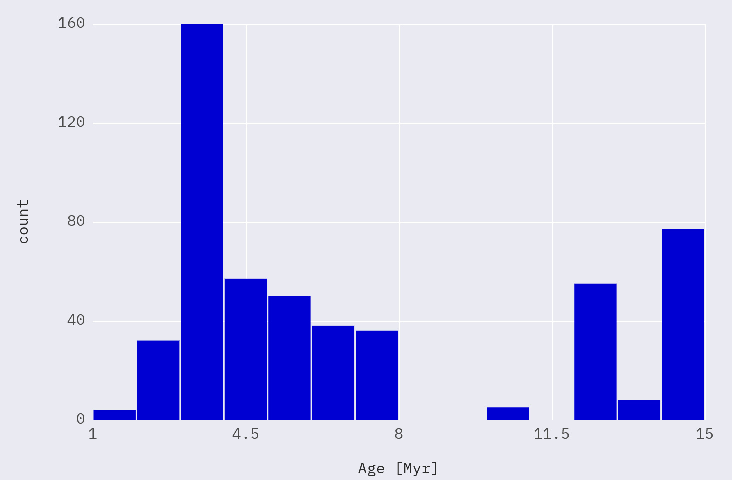
\includegraphics[width=0.6\linewidth]{figures/age_hist.pdf}
    \caption{}
    \label{fig:app_age_hist}
\end{figure}


\section{Velocity Vector Visualizations}
\label{app:vectorplots}

Figure~\ref{fig:app_uvw_vectors} shows the full three-dimensional velocity vectors
$(U, V, W)$ of the subsample of 180 stars for which a radial-velocity measurement is
available, plotted at their respective three-dimensional positions within the
reconstruction volume. Figure~\ref{fig:app_pm_vectors} instead shows the tangential
proper-motion vectors of the full 557-star catalog, projected onto the plane of the sky
as seen from the Sun; since these are angular rather than physical velocities, no
distance information is encoded in this second plot.

\begin{figure}[h!]
    \centering
    \begin{subfigure}[b]{0.9\linewidth}
        \centering
        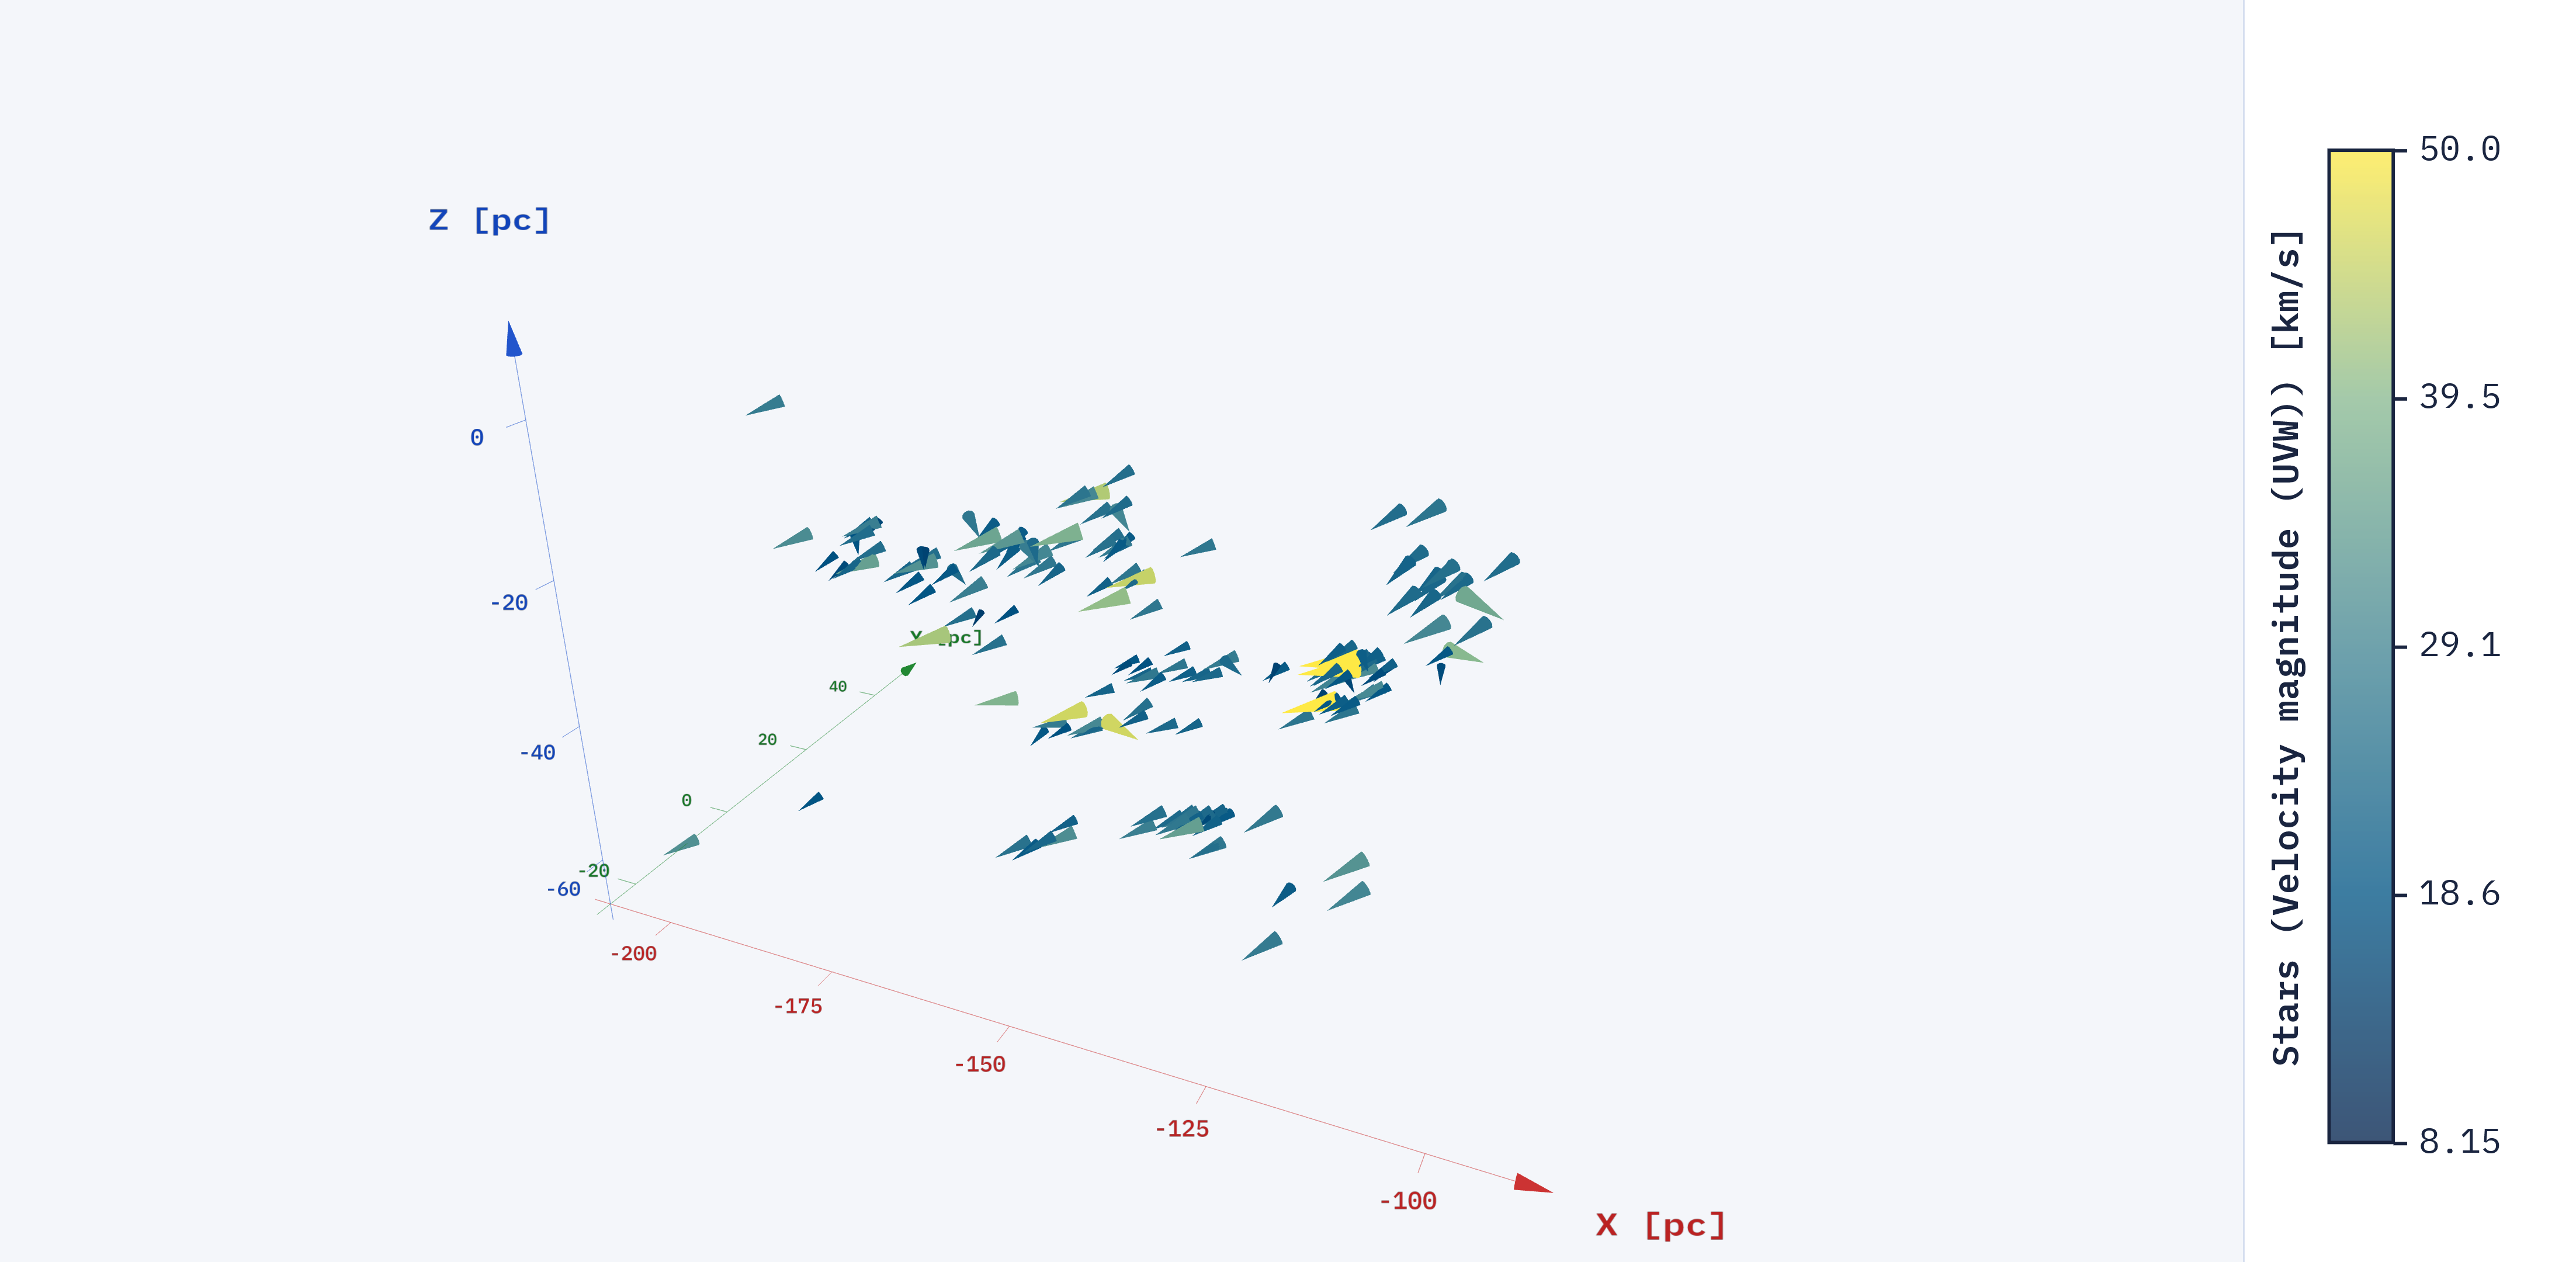
\includegraphics[width=\linewidth]{figures/UVW.png}
        \caption{Full three-dimensional velocity vectors of the radial-velocity
            subsample, shown at their three-dimensional positions.}
        \label{fig:app_uvw_vectors}
    \end{subfigure}
    \vspace{1em}
    \begin{subfigure}[b]{0.9\linewidth}
        \centering
        
\includegraphics[width=\linewidth]{figures/test.png}
        \caption{Proper-motion vectors of the full catalog, projected onto the sky.}
        \label{fig:app_pm_vectors}
    \end{subfigure}
    \caption{Vector-based illustrations of the two velocity data modalities entering the
        reconstruction: full three-dimensional space velocities of the radial-velocity
        subsample (top) versus sky-projected proper motions of the full sample (bottom).}
    \label{fig:app_vectors}
\end{figure}



\end{document}